\documentclass[a4paper,7pt]{article}

\usepackage{graphicx}
\usepackage{verbatim}		%Include it to use a comment
\usepackage{hyperref}		%Used for creating hrref

\title{Project Report}
\begin{document}
\author{Gaurav}


\maketitle
\date
\abstract{This is a report abstract}


\newpage
\tableofcontents		%Used for contents



\newpage		%This will insert a new page
This is my first latex document
" hello  world "
\section{Introduction}
Intro is here		
Let $\mathbf{u}$,$\mathbf{v}$ and $\mathbf{w}$ be three
vectors in ${\mathbf R}^3$. The volume~$V$ of the
parallelepiped with corners at the points
$\mathbf{0}$, $\mathbf{u}$, $\mathbf{v}$,
$\mathbf{w}$, $\mathbf{u}+\mathbf{v}$,
$\mathbf{u}+\mathbf{w}$, $\mathbf{v}+\mathbf{w}$
and $\mathbf{u}+\mathbf{v}+\mathbf{w}$
is given by the formula
\[ V = (\mathbf{u} \times \mathbf{v}) \cdot \mathbf{w}.\]


The roots of a quadratic polynomial $a x^2 + bx + c$ with
$a \neq 0$ are given by the formula
\[ \frac{-b \pm \sqrt{b^2 - 4ac}}{2a} \]





\begin{comment}
     This is also a comment !!..
\end{comment}


\[f(x)=2x+\frac{2x-7}{x^2+4}\]





\includegraphics[scale=0.4]{4.jpg}
\section{Theory}
theory is here
\newline				%To give a newline
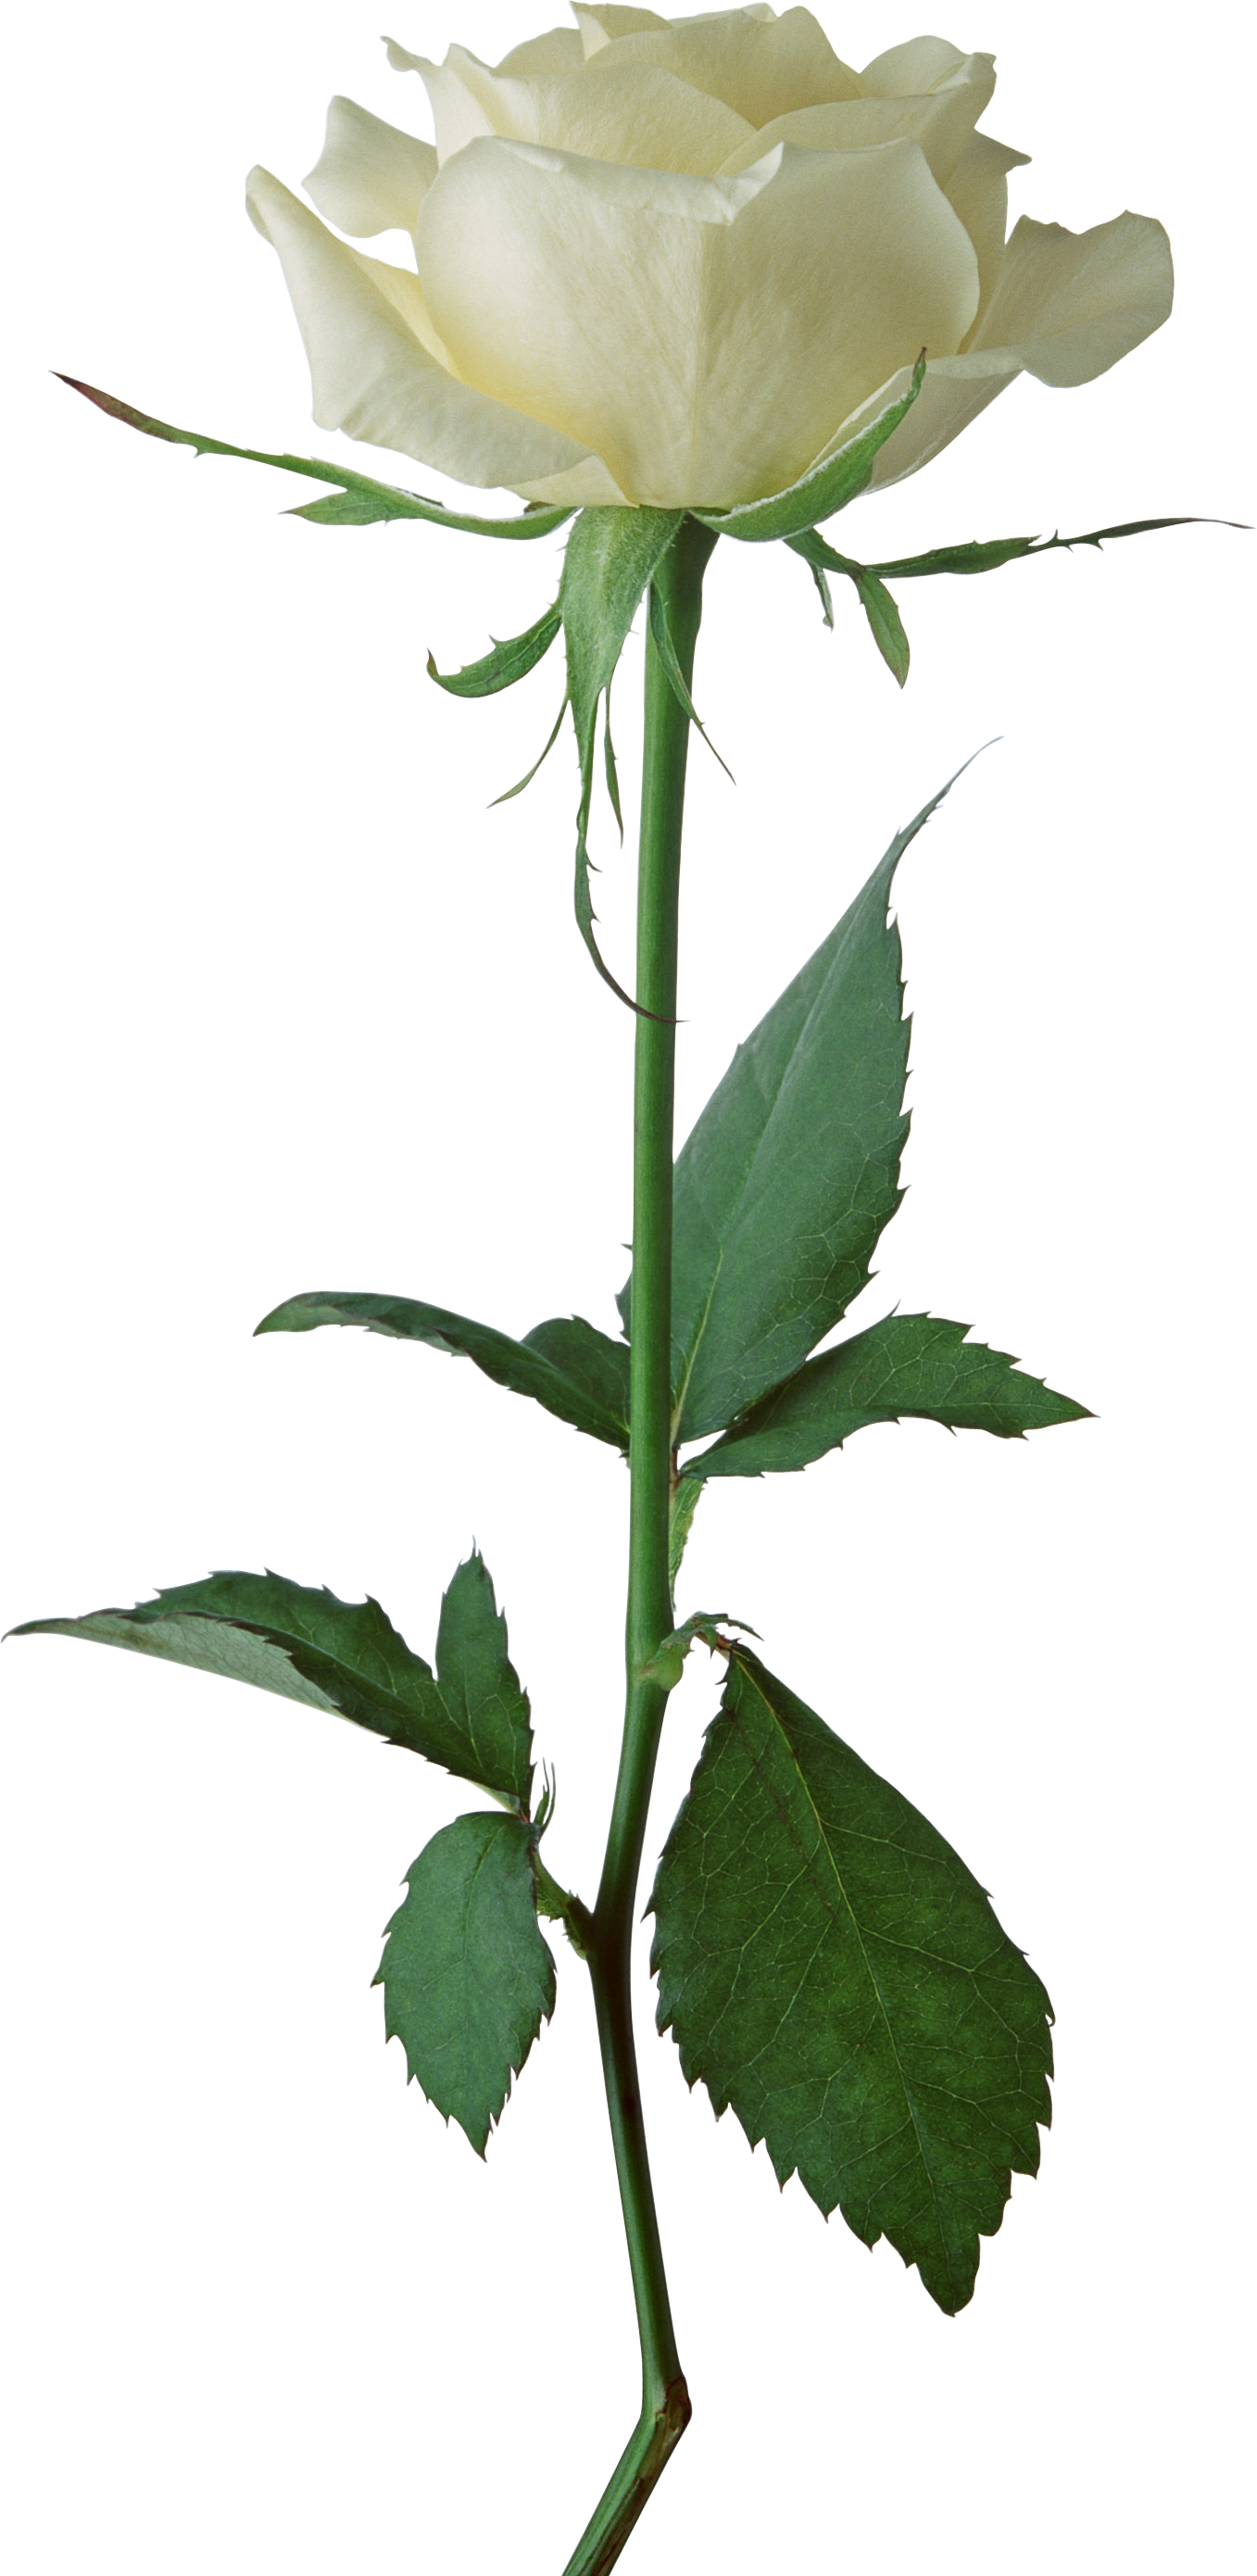
\includegraphics[scale=0.35]{006.png}






\section{Equations}
\begin{equation}
     x1=sinx()
     \label{sin}
\end{equation}
\begin{equation}
     x2=cos(x)
     \label{cos}
\end{equation}


\[f(x)=x^2	\] 
\(g(x)=x^3	\) and we have \(h(x)=x^4	\)
$ w     is    9 $
\newline

\[f(x_1,x_2,\ldots,x_n)=x_1^2+x_2^2+\ldots+x_n^2\]





\section{Conclusions}
Here is the conclusion
Equation \ref{sin} is for finding sine
Equation \ref{cos} is for finding cosine\newline
And some mine equations are:\\
The roots of the cubic polynomial of the form $x^3 -3px -2q$ are given by the formula \newline
\[f(x)=\sqrt[3]{q+\sqrt{q^2 - p^3}}+\sqrt[3]{q-\sqrt{q^2}}\]



\section{New}


\[ \lim_{x \to +\infty} \frac{3x^2 +7x^3}{x^2 +5x^4} = 3.\]

\[ \sum_{k=1}^n k^2 = \frac{1}{2} n (n+1).\]

\[ \int_a^b f(x)\,dx.\]

\[ \int_0^{+\infty} x^n e^{-x} \,dx = n!.\]
\[ \int \cos \theta \,d\theta = \sin \theta.\]
\[ \int_{x^2 + y^2 \leq R^2} f(x,y)\,dx\,dy
     = \int_{\theta=0}^{2\pi} \int_{r=0}^R
f(r\cos\theta,r\sin\theta) r\,dr\,d\theta.\]

\[ \int_0^R \frac{2x\,dx}{1+x^2} = \log(1+R^2).\]


\end{document}
